\documentclass[conference]{IEEEtran}
\usepackage{cite}
\usepackage{amsmath,amssymb,amsfonts}
\usepackage{algorithmic}
\usepackage{graphicx}
\usepackage{textcomp}
\usepackage{xcolor}
\usepackage{amsmath}
\usepackage{amsfonts}
\usepackage{amssymb}
\usepackage{mathtools}
\usepackage{amsthm}
\def\BibTeX{{\rm B\kern-.05em{\sc i\kern-.025em b}\kern-.08em
		T\kern-.1667em\lower.7ex\hbox{E}\kern-.125emX}}


\newtheorem{algorithm}{Algorithm}
\newtheorem{definition}{Definition}
\newtheorem{lemma}{Lemma}
\newtheorem{theorem}{Theorem}
\newtheorem{remark}{Remark}

\begin{document}

\title{Short CAGD}

\author{\IEEEauthorblockN{Ida Hönigmann}}

\maketitle

\section{General}

\begin{definition}[Combinations]
	\hspace{1cm}
	\begin{table}[h!]
		\begin{tabular}{lll}
			Linear Combination & $\sum_{i=1}^{n} \lambda_i v_i$ & $v_i \in \mathbb{R}^d, \lambda_i \in \mathbb{R}$\\
			Affine Combination & $\sum_{i=1}^{n} \lambda_i v_i$ & above and $\sum_{i=1}^{n} \lambda_i = 1$\\
			Convex Combination & $\sum_{i=1}^{n} \lambda_i v_i$ & above and $\forall i: \lambda_i \geq 0$\\
		\end{tabular}
	\end{table}	
\end{definition}

\begin{definition}[Affine Transformation]
	\begin{align*}
		\alpha: \mathbb{R}^n \rightarrow \mathbb{R}^m \text{ with }\\
		\exists l: \mathbb{R}^n \rightarrow \mathbb{R}^m \text{ ... linear } \exists v \in \mathbb{R}^m : \alpha(x) = l(x) + v
	\end{align*}
\end{definition}

\begin{definition}[Convex Set, Convex Hull]
	\begin{align*}
		M ... convex \iff \forall x,y \in M \forall t \in [0, 1] : tx + (1-t)y \in M\\
		conv(M) := \{\sum_{i=0}^{n} \lambda_i v_i: v_i \in M, \lambda_i \geq 0, \sum_{i=0}^{n} \lambda_i = 1, n\in \mathbb{N}\}
	\end{align*}
\end{definition}

\begin{definition}[Described by Same Parameter]
	$\phi$ is described over $f$, $\tilde{f}$ by the same parameter, iff $f,\tilde{f}$ ... bij.
	\begin{align*}
		\phi: f(U) \rightarrow \tilde{f}(U), x \mapsto \tilde{f} \circ f^{-1}(x)
	\end{align*}
\end{definition}
	
\section{Parameterized Curves}

\begin{definition}[Tangential Vector, Velocity]
	\begin{align*}
		tangent := \dot{c}(t) && vel := ||\dot{c}(t)||
	\end{align*}
\end{definition}

\begin{definition}[Regular, Singular]
	\begin{align*}
		regular \iff \dot{c}(t) \neq 0 && singular \iff \dot{c}(t) = 0
	\end{align*}
\end{definition}

\begin{definition}[Curvature, Torsion]
	\begin{align*}
		\kappa(t) := \frac{\det(\dot{c}(t), \ddot{c}(t))}{||\dot{c}(t)||^3} && \text{ for } c:I \rightarrow \mathbb{R}^2\\
		\kappa(t) := \frac{||\dot{c}(t) \times \ddot{c}(t)||}{||\dot{c}(t)||^3} && \text{ for } c:I \rightarrow \mathbb{R}^3\\
		\tau(t) := \frac{\det(\dot{c}(t), \ddot{c}(t), \dddot{c}(t))}{||\dot{c}(t) \times \ddot{c}(t)||^2} && \text{ for } c:I \rightarrow \mathbb{R}^3
	\end{align*}
\end{definition}

\begin{definition}[Vertex]
	$c(t)$ with $\dot{\kappa}(t) = 0$
\end{definition}
	
\begin{definition}[Length]
	\begin{align*}
		L(c) := \int_I ||\dot{c}(t)|| dt
	\end{align*}
\end{definition}

\begin{definition}[Isometric = Preserving Length]
	\begin{align*}
		\forall c:I\rightarrow M: L(\phi(c)) = L(c)
	\end{align*}
\end{definition}

\section{Bezier Curves}

\begin{algorithm}[of de Casteljou]
	\begin{align*}
		b_i^0(t):= b_i && b_i^j(t) := (1-t)b_i^{j-1}(t) + t b_{i+1}^{j-1}(t) && b(t) := b_0^n(t)
	\end{align*}
\end{algorithm}

\begin{definition}[Bernstein Polynomials]
	\begin{align*}
		B_i^n(t) := \binom{n}{i} t^i (1-t)^{n-i} \in \mathbb{R}[t]
	\end{align*}
\end{definition}

\begin{theorem}[Bernstein Representation of Bezier Curve]
	\begin{align*}
		b_i^j(t) = \sum_{l=0}^{j} B_l^j(t) b_{i+l}
	\end{align*}
\end{theorem}

\begin{proof}
	Induction over $j$ using the fact that\\
	$B_l^j(t) = (1-t)B_l^{j-1}(t) + t B_{l-1}^{j-1}(t)$.
\end{proof}

\begin{lemma}[Properties of Bernstein Polynomials]
	\begin{align*}
		\sum_{i=1}^{n} B_i^n(t) = 1\\
		t \in [0, 1] \implies B_i^n(t) \geq 0\\
		B_i^n(\alpha t) = \sum_{j=0}^{n} B_i^j(\alpha) B_j^n(t)\\
		\{B_0^n(t), ..., B_n^n(t)\} \text{ forms a basis of } \Pi_n
	\end{align*}
\end{lemma}


\begin{lemma}[Endpoint Interpolating]
	\begin{align*}
		b(0) = b_0 && b(1) = b_n
	\end{align*}
\end{lemma}

\begin{lemma}[Tangent of Bezier Curves]
	\begin{align*}
		\dot{b}(t) = n(b_1^{n-1}(t) - b_0^{n-1}(t))
	\end{align*}
\end{lemma}

\begin{proof}
	Calculation using the fact that\\
	$\frac{d}{dt} B_i^n(t) = n (B_{i-1}^{n-1}(t) - B_i^{n-1}(t))$.
\end{proof}

\begin{theorem}[Invariant under Affine Transformations]
	\begin{align*}
		\alpha(b(t)) = \sum_{i=0}^{n} B_i^n(t) \alpha(b_i)
	\end{align*}
\end{theorem}

\begin{theorem}[Bezier Curve is in Convex Hull]
	\begin{align*}
		t \in [0, 1] \implies b(t) \in conv(\{b_0, ..., b_n\})
	\end{align*}
\end{theorem}

\begin{theorem}[Bezier Curve is Symmetric]
	\begin{align*}
		b(t) \text{ from points } b_0, ..., b_n && \tilde{b}(t) \text{ from points } b_n, ..., b_0\\
		\implies b(t) = \tilde{b}(1-t)
	\end{align*}
\end{theorem}

\newpage
\begin{theorem}[Sub-division property]
	\begin{align*}
		\tilde{b}(t) := b(\alpha t) && \hat{b}(t) := b((1-\alpha)t + \alpha)
	\end{align*}
	Then
	\begin{align*}
		\tilde{b} \text{ from points } b_0^0(\alpha), ..., b_0^n(\alpha)\\
		\hat{b} \text{ from points } b_0^n(\alpha), b_1^{n-1}(\alpha), ..., b_n^0(\alpha)
	\end{align*}
	and ''gluing'' them together results in $b(t)$.
\end{theorem}

\begin{theorem}
	Every polynomial curve is a Bezier curve.
\end{theorem}

\begin{theorem}[Corner-cutting]
	\begin{align*}
		P_0 := (b_0, ..., b_n) && P_n := \text{ sub-divide $n$ times with $n=1/2$ }\\
		\implies P_n \rightarrow b(t)
	\end{align*}
\end{theorem}

\section{B-Spline and NURBS}

\begin{definition}[B-Spline]
	Composition of Bezier Curves.
\end{definition}

\begin{definition}[B-Spline Base Functions]
	\begin{align*}
		\alpha_i^r(t) := \begin{cases}
							\frac{t-t_i}{t_{i+r}-t_i} & t_{i+r}-t_i \neq 0,\\
							0, & \text{ else}
						\end{cases}\\
		N_i^0(t) := \begin{cases}
						1, & t \in [t_i, t_{i+1})\\
						0, & \text{ else}
					\end{cases}\\
		N_i^r(t) := \alpha_i^r(t) N_i^{r-1}(t) + (1-\alpha_i^r(t)) N_{i+1}^{r-1}(t)
	\end{align*}
\end{definition}

\begin{lemma}[Properties of B-Spline Base Functions]
	\begin{align*}
		\sum_{i=0}^{m} N_i^n(t) = 1 && N_i^n(t) \geq 0
	\end{align*}
\end{lemma}

\begin{theorem}[B-Spline Representation]
	$m$ ... number control points, $n$ ... degree, $T=(t_0, ..., t_{m+n+1})$ ... knot vector with $t_i \leq t_{i+1}$, $t_i < t_{i+n+1}$
	
	\begin{align*}
		s(t) = \sum_{i=0}^{m} N_i^n(t) c_i
	\end{align*}
\end{theorem}

\begin{definition}[NURBS]
	Construction by:\\
	\begin{enumerate}
		\item homogenize control points
		\item scale by weight
		\item construct B-Spline
		\item project back onto $1\times\mathbb{R}^d$
		\item dehomogenize
	\end{enumerate}
\end{definition}

\begin{lemma}
	B-Spline curve with $m=n$ is a Bezier curve.\\
	NURBS with $w_i = w$ is a B-Spline.
\end{lemma}

\begin{remark}
	$w_i$ bigger $\implies$ curve is attracted towards $c_i$.
\end{remark}

\begin{remark}
	NURBS can construct conic sections (such as circles).
\end{remark}

\begin{lemma}
	B-Spline and NURBS are both affine invariant.
\end{lemma}

\section{Free Form Surfaces}

\begin{definition}[Free Form Surface]
	$b_{00}, b_{01}, ..., b_{mn} \in \mathbb{R}^d$, $g(s) = \sum_{i=0}^{m} D_i(s) p_i$, $h(t) = \sum_{j=0}^{n} E_j(t) q_j$
	
	\begin{align*}
		f(s,t) := \sum_{i=0}^{m} \sum_{j=0}^{n} D_i(s) E_j(t) b_{ij}
	\end{align*}
\end{definition}

\begin{remark}
	Many same theorems as in Bezier, B-Spline and NURBS hold.
\end{remark}

\section{Subdivision of Curves}

\begin{algorithm}[Chaikin]
	copy once, average twice
	
%	\begin{figure}[h!]
%		\centering
%		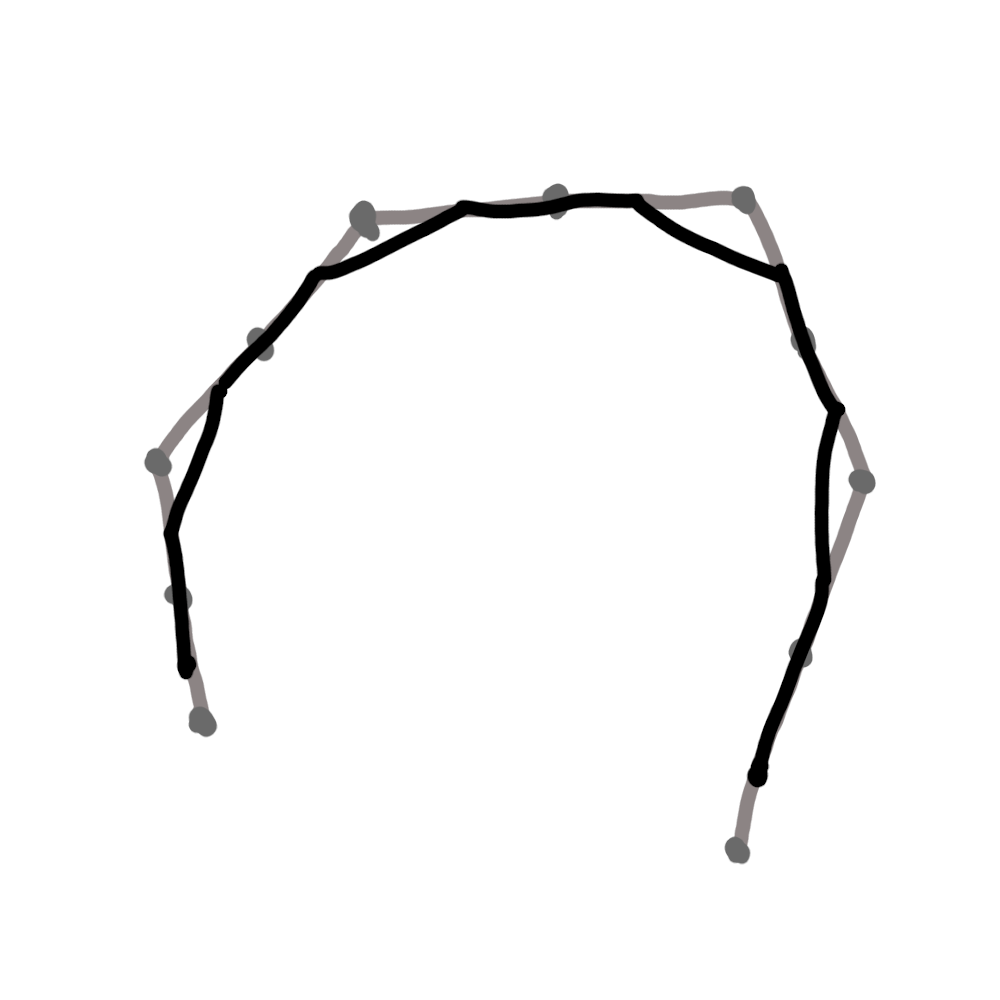
\includegraphics[width=0.4\linewidth]{figures/chaikin_short}
%		\caption{Chaikin}
%	\end{figure}
	
	\begin{itemize}
		\item $\rightarrow$ quadratic B-Spline
		\item approximating
		\item affine invariant
		\item linear precision
	\end{itemize}
\end{algorithm}

\begin{algorithm}[Lane-Riesenfeld]
	copy once, average $n$ times
	
%	\begin{figure}[h!]
%		\centering
%		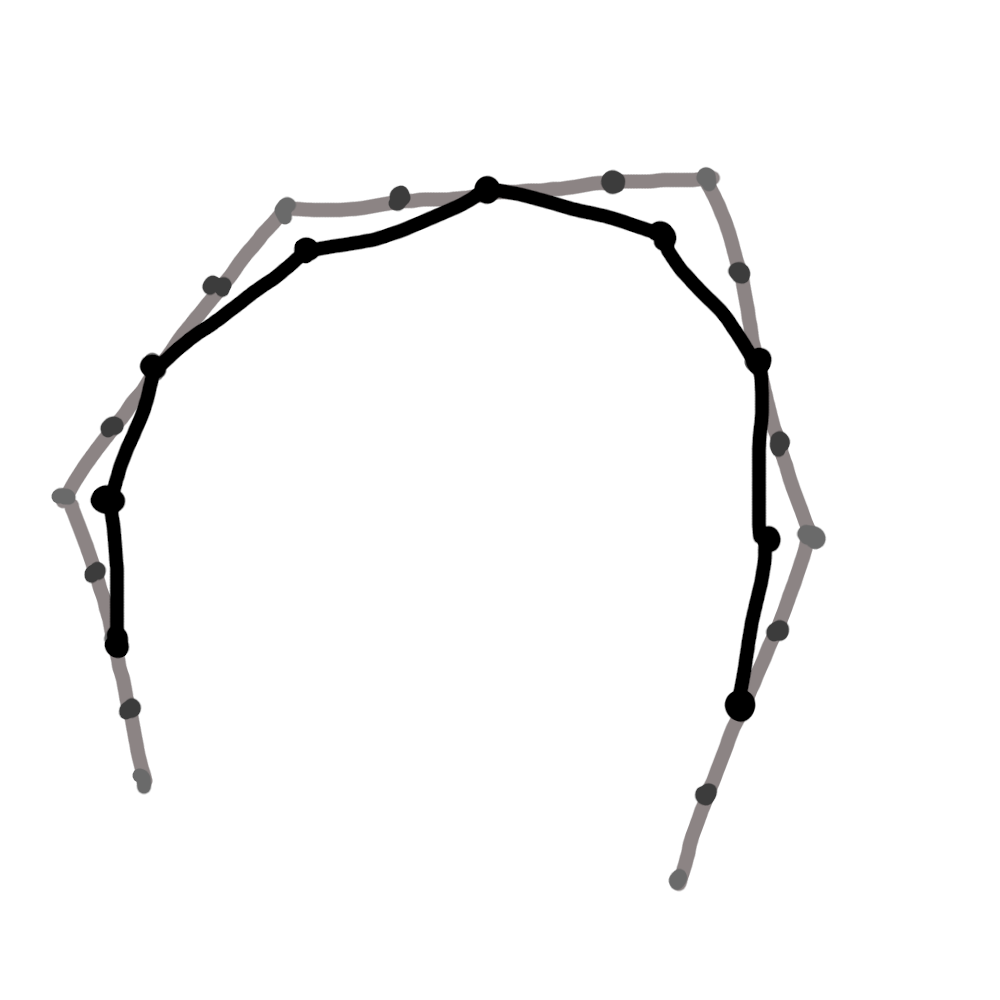
\includegraphics[width=0.4\linewidth]{figures/lane_riesenfeld_short}
%		\caption{Lane-Riesenfeld}
%	\end{figure}
	
	\begin{itemize}
		\item $\rightarrow$ B-Spline of degree $n$
		\item approximating
		\item affine invariant
		\item linear precision
	\end{itemize}
\end{algorithm}

\begin{algorithm}[Four Point Scheme]
	$p_i^0 := p_i$\\
	$p_i^l := -\frac{1}{16} p_{i-1}^{l-1} + \frac{9}{16} p_i^{l-1} + \frac{9}{16} p_{i+1}^{l-1} - \frac{1}{16} p_{i+2}^{l-1}$
	
%	\begin{figure}[h!]
%		\centering
%		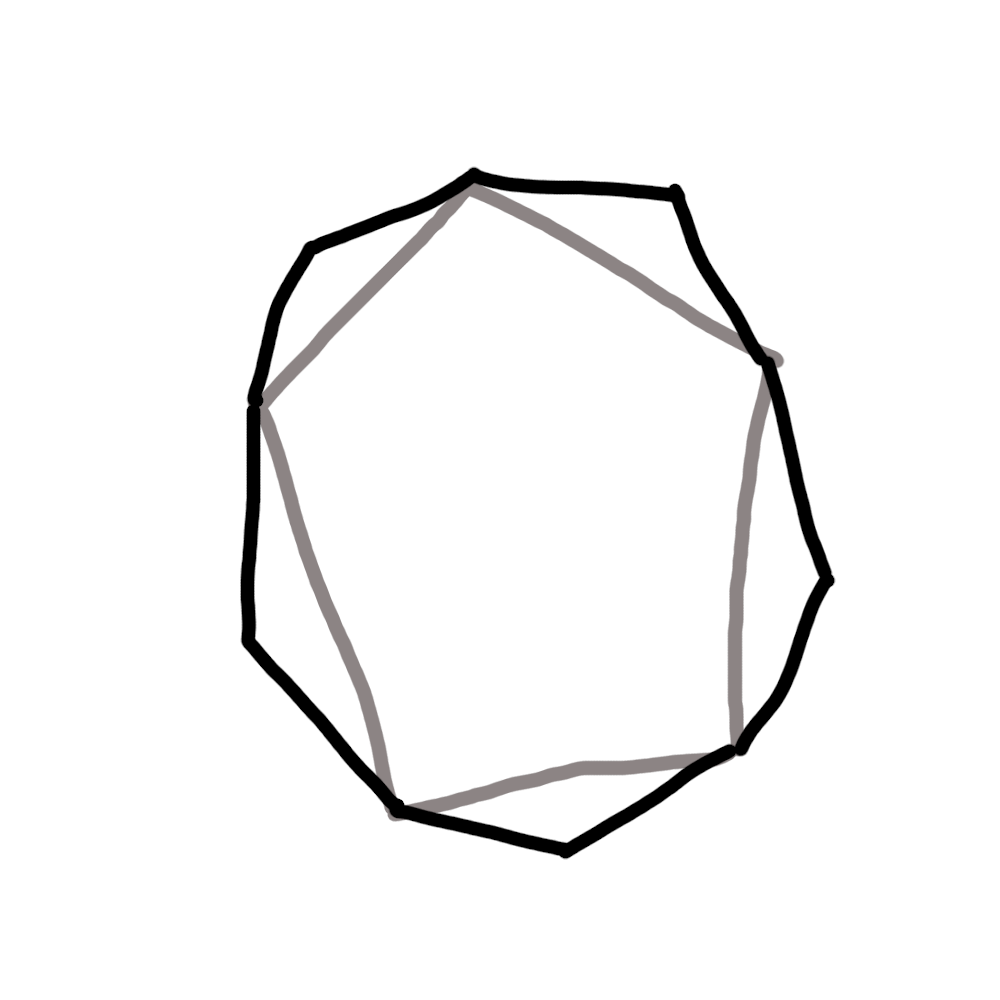
\includegraphics[width=0.4\linewidth]{figures/four_point_short}
%		\caption{Four Point Scheme}
%	\end{figure}
	
	\begin{itemize}
		\item $\rightarrow C^1$ curve
		\item interpolating
		\item affine invariant
		\item linear precision
	\end{itemize}
\end{algorithm}

\section{Subdivision of Meshes}

\begin{algorithm}[Loop]
	triangle mesh
	
	\begin{figure}[h!]
		\centering
		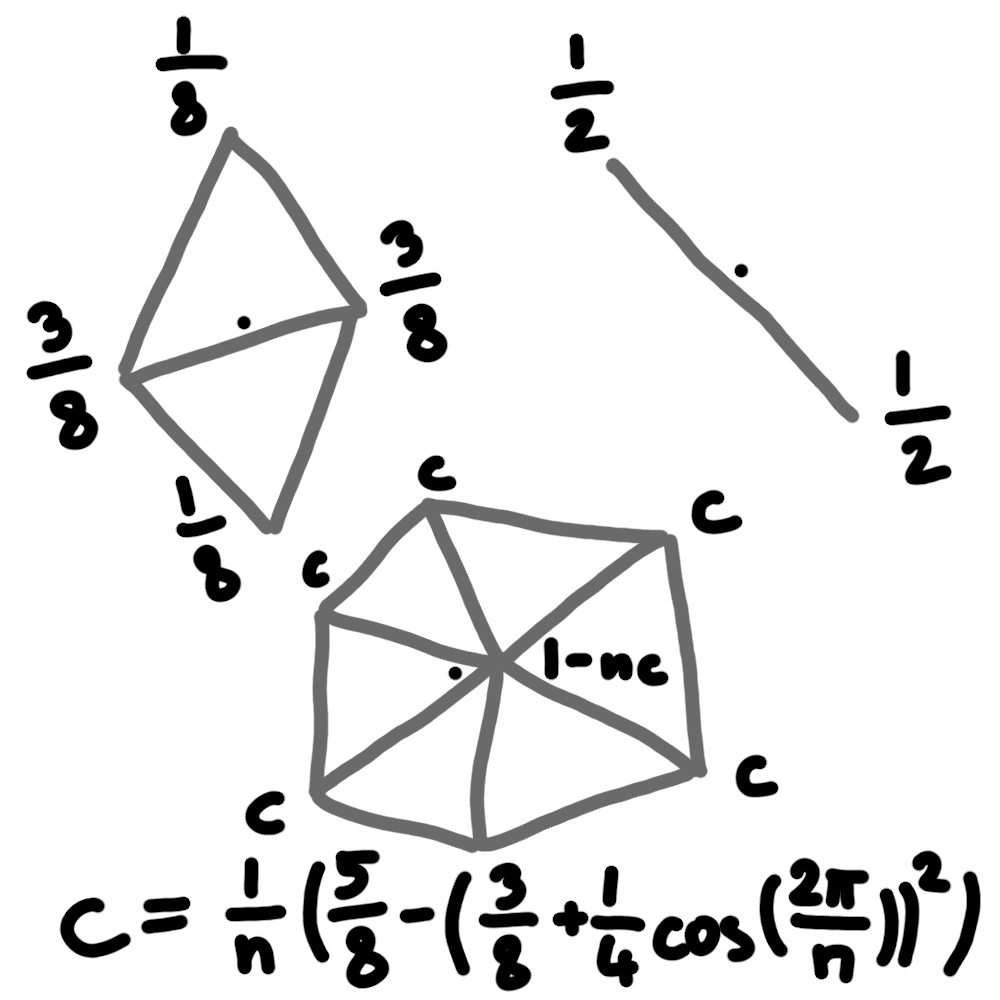
\includegraphics[width=0.4\linewidth]{figures/loop_short}
		\caption{Loop}
	\end{figure}
	
	\begin{itemize}
		\item $\rightarrow C^2$ in generic ($n=6$) case
		\item $\rightarrow C^1$ otherwise
		\item approximating
		\item face splitting
	\end{itemize}
\end{algorithm}

\newpage
\begin{algorithm}[Modified Butterfly]
	triangle mesh
	
	\begin{figure}[h!]
		\centering
		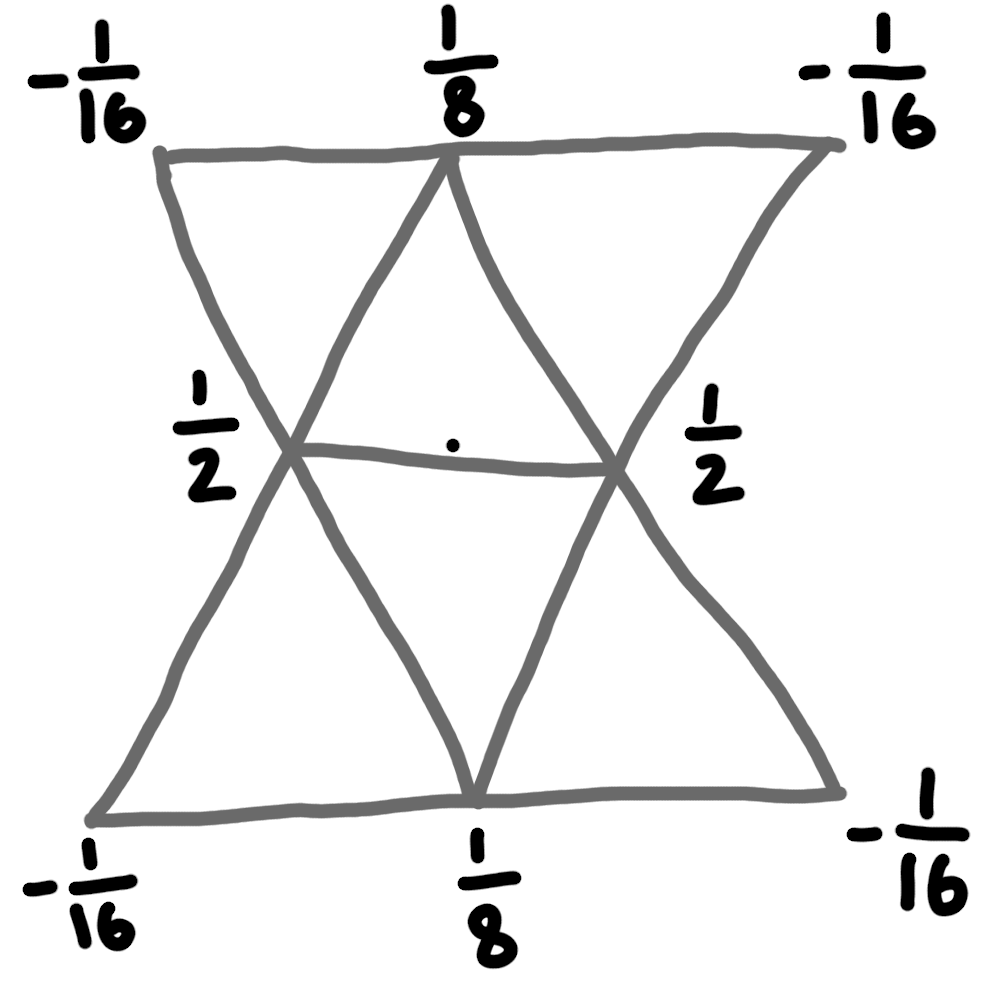
\includegraphics[width=0.4\linewidth]{figures/modified_butterfly_short}
		\caption{Modified Butterfly}
	\end{figure}
	
	\begin{itemize}
		\item $\rightarrow C^1$ surface
		\item interpolating
		\item face splitting
	\end{itemize}
\end{algorithm}

\begin{algorithm}[Catmull Clark]
	square mesh
	
	\begin{figure}[h!]
		\centering
		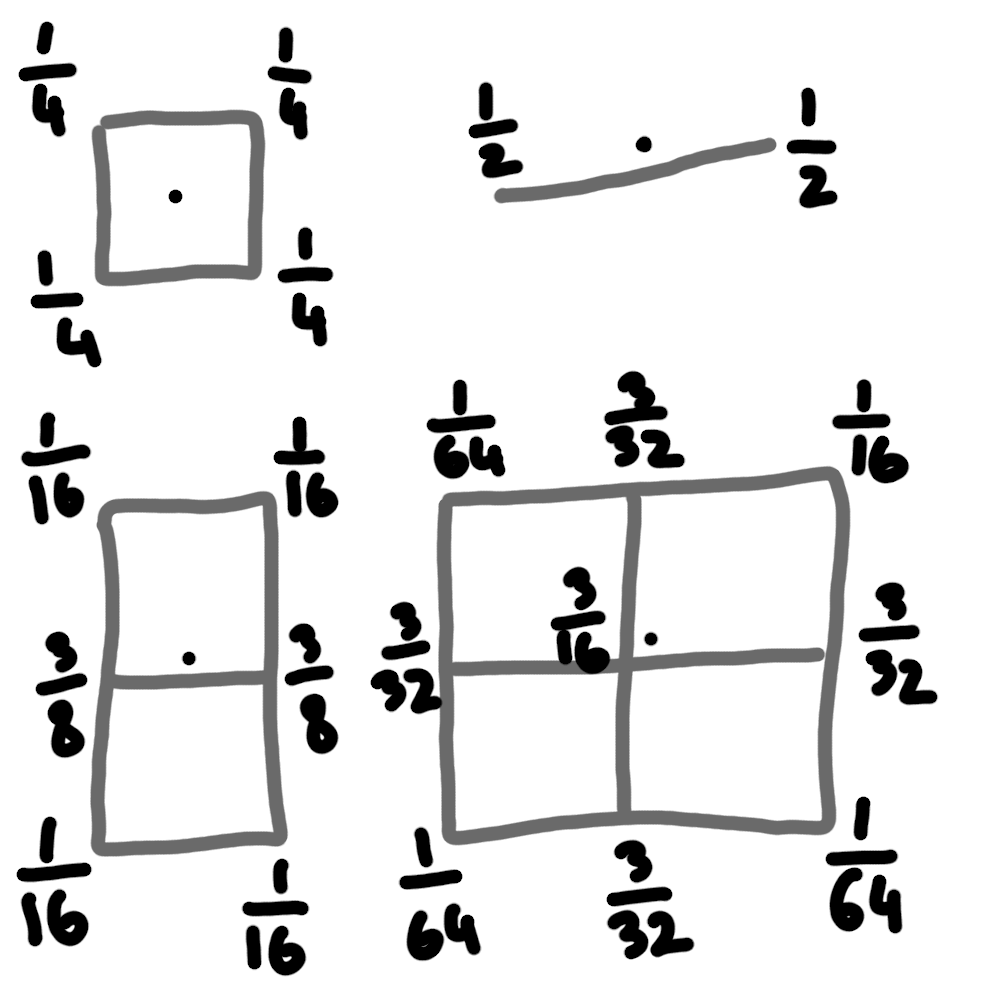
\includegraphics[width=0.4\linewidth]{figures/catmull_clark_short}
		\caption{Catmull Clark}
	\end{figure}
	
	\begin{itemize}
		\item $\rightarrow C^2$ in generic ($n=4$) case
		\item approximating
		\item face splitting
	\end{itemize}
\end{algorithm}

\begin{algorithm}[Doo Sabin]
	any mesh
	
	\begin{figure}[h!]
		\centering
		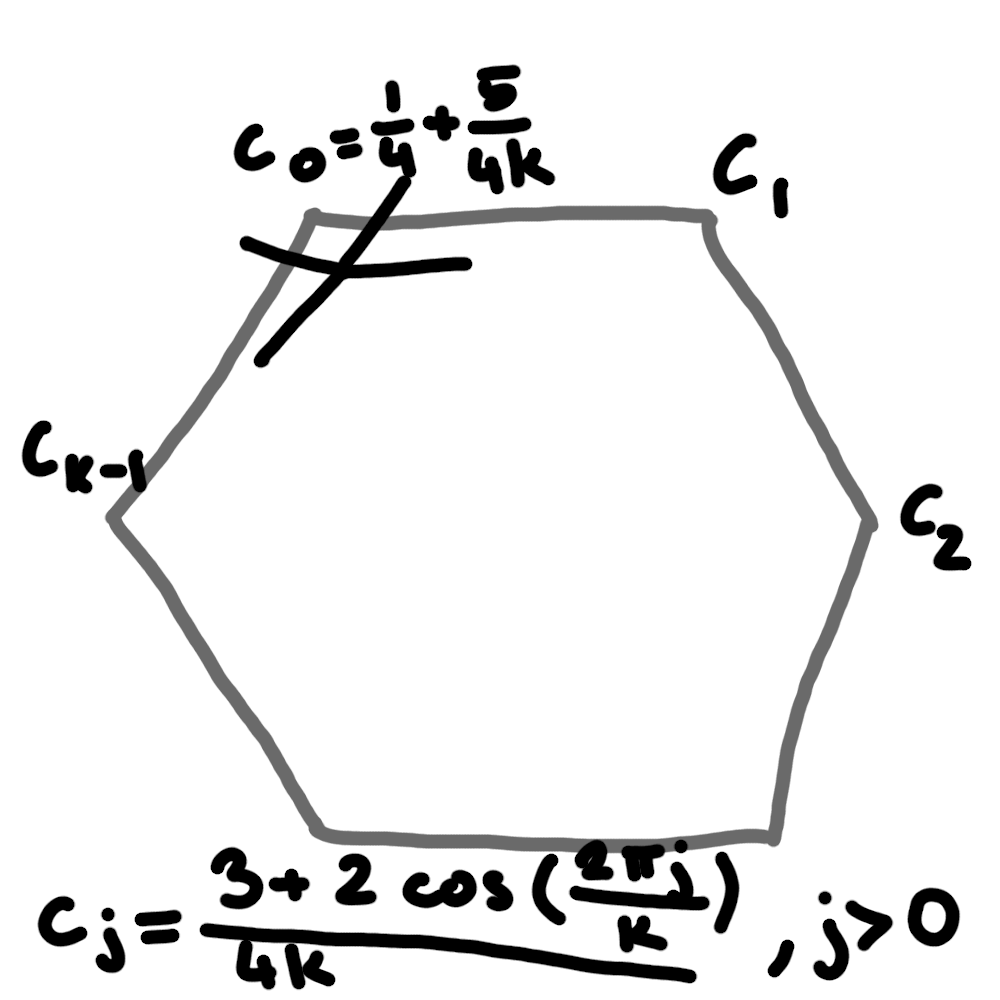
\includegraphics[width=0.4\linewidth]{figures/doo_sabin_short}
		\caption{Doo Sabin}
	\end{figure}
	
	\begin{itemize}
		\item $\rightarrow C^1$ surface
		\item approximating
		\item vertex splitting
	\end{itemize}
\end{algorithm}

\begin{algorithm}[Kobbelt]
	square mesh
	
%	\begin{figure}[h!]
%		\centering
%		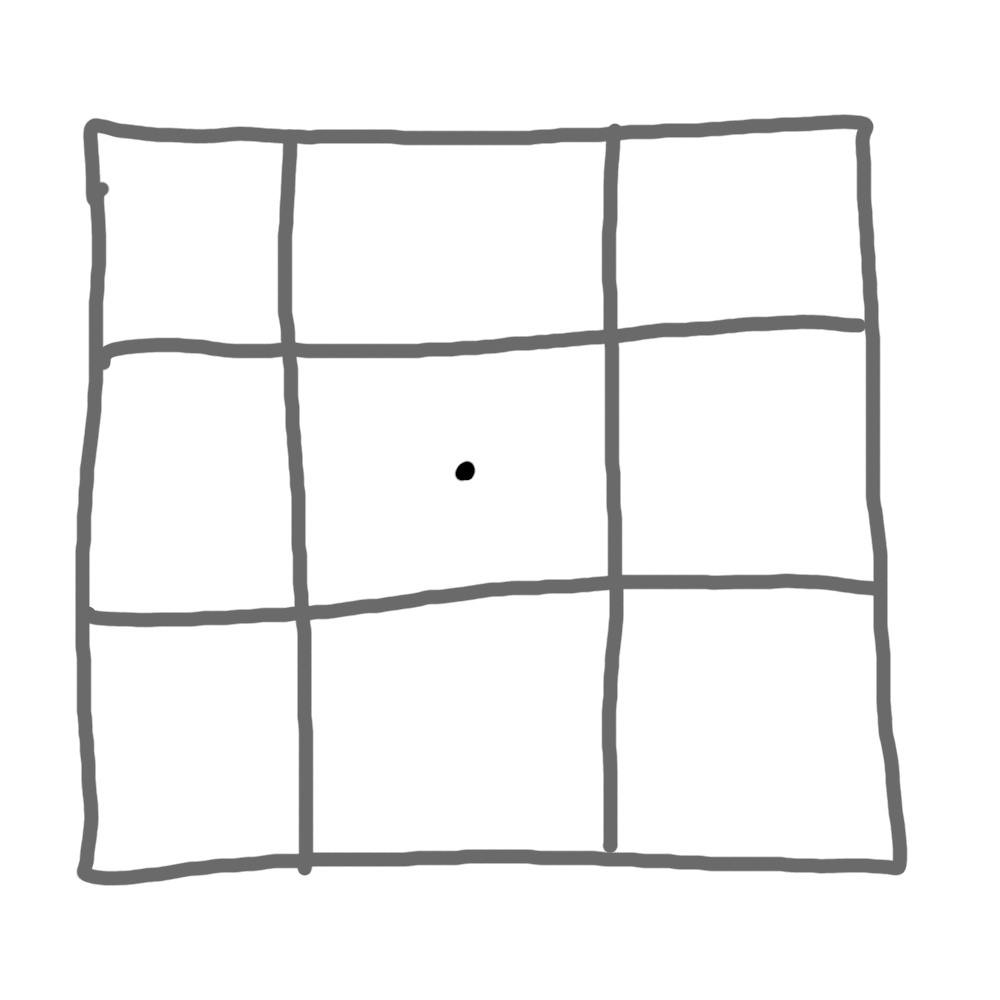
\includegraphics[width=0.4\linewidth]{figures/kobbelt_short}
%		\caption{Kobbelt}
%	\end{figure}
	
	four point scheme horizontal or vertical, then four point scheme on results
	
	\begin{itemize}
		\item $\rightarrow C^1$ surface
		\item interpolating
		\item face splitting
	\end{itemize}
\end{algorithm}

\section{Conformal Pattern Matching}

\begin{definition}[Möbius Transformation]
	Composition of reflections on hyper-sphere.
\end{definition}

\begin{definition}[Reflection on Sphere]
	\begin{align*}
		\tilde{\omega} := \frac{r^2}{||\omega||^2} \omega && \tilde{0} := \infty && \tilde{\infty} := 0
	\end{align*}
\end{definition}

\begin{definition}[Cross Ratio]
	\begin{align*}
		DV(a,b,c,d) := \frac{(a-b)(c-d)}{(b-c)(d-a)} \in \mathbb{C}
	\end{align*}
\end{definition}

\begin{theorem}
	Cross Ratio is invariant under Möbius transformations.
\end{theorem}

\begin{theorem}
	Möbius transformations preserve angles (=conformal) and circles.
\end{theorem}

\begin{definition}[Discrete Metric]
	\begin{align*}
		L:E \rightarrow \mathbb{R}_{\geq 0}\\
		\forall f \in F: l_{ij} \leq l_{jk} + l_{ki}, l_{jk} \leq l_{ki} + l_{ij}, l_{ki} \leq l_{ij} + l_{jk}, l_{ij} = l_{ji}
	\end{align*}
\end{definition}

\begin{definition}[Discrete Conform Equivalent]
	
	$T, \tilde{T}$ .. combinatorial equivalent triangle meshes with
	
	\begin{align*}
		\exists \lambda: E \rightarrow \mathbb{R}_{\geq 0} \forall (i,j) \in E: \tilde{l}_{ij} = \lambda_i \lambda_j l_{ij}
	\end{align*}
\end{definition}

\begin{definition}[Length Cross Ratio]
	\begin{align*}
		LDV(v_i, v_j, v_k, v_m) := \frac{l_{ij} l_{km}}{l_{jk} l_{mi}}
	\end{align*}
\end{definition}

\begin{lemma}
	$(T,l), (\tilde{T}, \tilde{l})$ are discrete conformal equivalent, iff $LDV(v_i, v_j, v_k, v_m) = LDV(\tilde{v}_i, \tilde{v}_j, \tilde{v}_k, \tilde{v}_m)$
\end{lemma}

\begin{lemma}
	$T$ ... triangle mesh, $l_{ij} := ||v_i - v_j||$, $m$ ... Möbius transformation, then $T, m(T)$ are discrete conformal equivalent.
\end{lemma}

\begin{theorem}
	Let $T$ be a triangle mesh and $\Phi_i \geq 0 \forall i \in V$.
	
	There exists a discrete conformal equivalent triangle mesh $\tilde{T}$, such that the sum of interior angles is $\Phi_i \forall i \in V$.
\end{theorem}

\begin{proof}
	There is a function $E(u)$ with $\frac{dE(u)}{du_i} = \Phi_i - \sum_{jk \in star(i)} \alpha_{jk}^i$, that can be extended to be a convex function on $\mathbb{R}^{\#V}$. Finding the critical points, that exist as $E(u)$ is convex, gives us the equivalent mesh $\tilde{T}$.
\end{proof}

\end{document}